% !TeX root = thesis.tex

\chapter{Conclusion}
\label{ch:conclusion}

The main purpose of this thesis has been to investigate different approaches towards optimising the test suite of a common software project. The concepts of \tsm{}, \tcs{} and \tcp{} have been introduced and accompanying algorithms have been presented. A novel client-server oriented framework for the latter approach has been proposed, as well as a new prioritisation algorithm. Finally, \velocity{} has been applied to the UGent Dodona project, proving its ability to predict test case failure and therefore reduce the execution time of the test suite.\\

\noindent A second purpose of this thesis was to gain useful insights into the behaviour of a typical test suite. These insights have been formulated as three additional research questions, to which answers have been provided in the previous chapter.

\section{Future work}
The proposed \velocity{} implementation in this thesis is currently able to prioritise a Gradle Java project using 10 available predictors and a meta predictor. While this is certainly functional, it is far from complete and multiple improvements can be added.

\subsection{Java Agent}
The existing Java Agent can be extended in multiple ways. The most prominent addition would be to allow test cases to be executed in parallel. At the moment of writing, this is not possible yet. In order to facilitate parallel testing, one must first decide how to schedule the prioritised test cases across multiple threads, since the execution time of a test case varies strongly. One possibility to perform this scheduling is to use the average execution time per test case, which is obtained from prior runs. Alternatively, this can be performed at runtime by using any existing inter-thread communication paradigm such as message passing. On the implementation side of parallelisation, the current \texttt{TestProcessor} should be adapted to inherit from the \texttt{MaxNParallelTestClassProcessor}. A thread pool should ideally be used to reduce the overhead of restarting a new thread for every test case.

\subsection{Predictions}
Further research and improvements to the predictors can be made on four different aspects.\\

\noindent The first enhancement is that currently the predictor does not discriminate between a unit test or an integration test. 
Recall that the scope of a unit test is limited to a small fraction of the application and that its execution time is ideally rather low. An integration test however usually takes longer to execute and tests multiple components of the application at once. The predictor could make use of this distinction and assume that a failure in a unit test has a high probability of resulting in a failed integration test as well, hence prioritising unit tests over integration tests.\\

\noindent Secondly, the prediction algorithms currently take into account which source code lines have either been modified or removed in order to prioritise affected test cases. Likewise, test cases of which the code has been modified should also be considered as candidates for prioritisation, as the changed test case might contain a bug as well.\\

\noindent A third and unexplored research opportunity is to investigate the joint performance of multiple prediction algorithms combined. This could be integrated with the existing meta predictor. Instead of assigning a score to the entire prediction, multiple predictions could be intermingled using predefined weights.\\

\noindent The final improvement is to take into account branch coverage in addition to the statement coverage which is currently used. This is a rather complex feature as not every coverage framework is capable of reporting accurately which branches have been covered and which ones have not. A suggested implementation would be to instrument the source code and rewrite every condition of every branch as separate \texttt{if}-statements.

\subsection{Meta predictor}
The proposed meta predictor increases the score of every predictor which predicted an above-average ranking and decreases the score of the other predictors. However, a possible problem with this approach is that the nature of the source code might evolve and change as time progresses. Using the current updating strategy it will take several test suite invocations for an alternative predictor to be preferred by the meta predictor. If a saturating counter would be used instead (\autoref{fig:saturating-counter}), this would be resolved much more quickly, allowing a more versatile meta predictor.

\begin{figure}[htbp!]
	\centering
	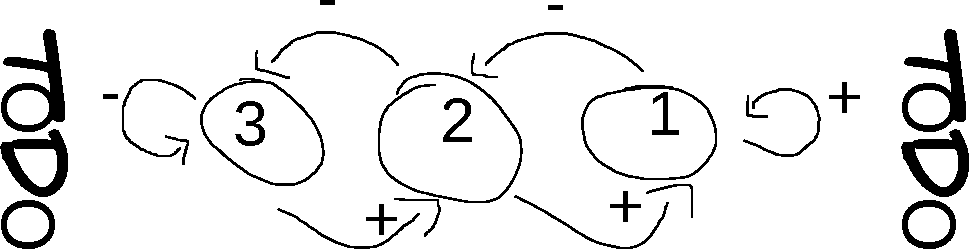
\includegraphics[width=\textwidth]{assets/images/saturating-counter.pdf}
	\caption{Saturating counter}
	\label{fig:saturating-counter}
\end{figure}

In addition to implementing a different update strategy, it might be worth to investigate the use of machine learning or linear programming models as a meta predictor, or even as a prediction algorithm.

\subsection{Final enhancements}
Finally, since some of the implemented algorithms are inherently \tsm{} algorithms rather than prioritisation algorithms, the framework might opt to not execute some test cases at all, whereas now the entire test suite is always executed.\\

\noindent Support for other programming languages and frameworks is possible by implementing new agents. The basic implementation is straightforward to restart the test suite after every executed test case, should test case reordering not be supported natively by the test framework.